
    \item Consider regular polygons with number of sides \( n = 3, 4, 5, \ldots \) as shown in the figure. The center of mass of all the polygons is at height \( h \) from the ground. They roll on a horizontal surface about the leading vertex without slipping and sliding as depicted. The maximum increase in height of the locus of the center of mass for each polygon is \( \Delta \). Then \( \Delta \) depends on \( n \) and \( h \) as
        \begin{tasks}(2)
            \task \( \Delta = h \sin^2\left(\frac{\pi}{n}\right) \)
            \task \( \Delta = h \left( \frac{1}{\cos\left(\frac{\pi}{n}\right)} - 1 \right) \)
            \task \( \Delta = h \sin \left(\frac{2\pi}{n}\right) \)
            \task \( \Delta = h \tan^2\left(\frac{\pi}{2n}\right) \)
        \end{tasks}


\begin{center}
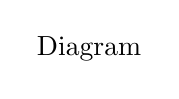
\begin{tikzpicture}
\node {Diagram};
\end{tikzpicture}
\end{center}